\documentclass[]{article}
\usepackage{lmodern}
\usepackage{amssymb,amsmath}
\usepackage{ifxetex,ifluatex}
\usepackage{fixltx2e} % provides \textsubscript
\ifnum 0\ifxetex 1\fi\ifluatex 1\fi=0 % if pdftex
  \usepackage[T1]{fontenc}
  \usepackage[utf8]{inputenc}
\else % if luatex or xelatex
  \ifxetex
    \usepackage{mathspec}
  \else
    \usepackage{fontspec}
  \fi
  \defaultfontfeatures{Ligatures=TeX,Scale=MatchLowercase}
\fi
% use upquote if available, for straight quotes in verbatim environments
\IfFileExists{upquote.sty}{\usepackage{upquote}}{}
% use microtype if available
\IfFileExists{microtype.sty}{%
\usepackage{microtype}
\UseMicrotypeSet[protrusion]{basicmath} % disable protrusion for tt fonts
}{}
\usepackage[left=1.1in, right=1.1in, top=1.1in, bottom=1.1in]{geometry}
\usepackage{hyperref}
\hypersetup{unicode=true,
            pdftitle={Stat 435 Lecture Notes 7},
            pdfauthor={Xiongzhi Chen; Washington State University},
            pdfborder={0 0 0},
            breaklinks=true}
\urlstyle{same}  % don't use monospace font for urls
\usepackage{color}
\usepackage{fancyvrb}
\newcommand{\VerbBar}{|}
\newcommand{\VERB}{\Verb[commandchars=\\\{\}]}
\DefineVerbatimEnvironment{Highlighting}{Verbatim}{commandchars=\\\{\}}
% Add ',fontsize=\small' for more characters per line
\usepackage{framed}
\definecolor{shadecolor}{RGB}{248,248,248}
\newenvironment{Shaded}{\begin{snugshade}}{\end{snugshade}}
\newcommand{\KeywordTok}[1]{\textcolor[rgb]{0.13,0.29,0.53}{\textbf{{#1}}}}
\newcommand{\DataTypeTok}[1]{\textcolor[rgb]{0.13,0.29,0.53}{{#1}}}
\newcommand{\DecValTok}[1]{\textcolor[rgb]{0.00,0.00,0.81}{{#1}}}
\newcommand{\BaseNTok}[1]{\textcolor[rgb]{0.00,0.00,0.81}{{#1}}}
\newcommand{\FloatTok}[1]{\textcolor[rgb]{0.00,0.00,0.81}{{#1}}}
\newcommand{\ConstantTok}[1]{\textcolor[rgb]{0.00,0.00,0.00}{{#1}}}
\newcommand{\CharTok}[1]{\textcolor[rgb]{0.31,0.60,0.02}{{#1}}}
\newcommand{\SpecialCharTok}[1]{\textcolor[rgb]{0.00,0.00,0.00}{{#1}}}
\newcommand{\StringTok}[1]{\textcolor[rgb]{0.31,0.60,0.02}{{#1}}}
\newcommand{\VerbatimStringTok}[1]{\textcolor[rgb]{0.31,0.60,0.02}{{#1}}}
\newcommand{\SpecialStringTok}[1]{\textcolor[rgb]{0.31,0.60,0.02}{{#1}}}
\newcommand{\ImportTok}[1]{{#1}}
\newcommand{\CommentTok}[1]{\textcolor[rgb]{0.56,0.35,0.01}{\textit{{#1}}}}
\newcommand{\DocumentationTok}[1]{\textcolor[rgb]{0.56,0.35,0.01}{\textbf{\textit{{#1}}}}}
\newcommand{\AnnotationTok}[1]{\textcolor[rgb]{0.56,0.35,0.01}{\textbf{\textit{{#1}}}}}
\newcommand{\CommentVarTok}[1]{\textcolor[rgb]{0.56,0.35,0.01}{\textbf{\textit{{#1}}}}}
\newcommand{\OtherTok}[1]{\textcolor[rgb]{0.56,0.35,0.01}{{#1}}}
\newcommand{\FunctionTok}[1]{\textcolor[rgb]{0.00,0.00,0.00}{{#1}}}
\newcommand{\VariableTok}[1]{\textcolor[rgb]{0.00,0.00,0.00}{{#1}}}
\newcommand{\ControlFlowTok}[1]{\textcolor[rgb]{0.13,0.29,0.53}{\textbf{{#1}}}}
\newcommand{\OperatorTok}[1]{\textcolor[rgb]{0.81,0.36,0.00}{\textbf{{#1}}}}
\newcommand{\BuiltInTok}[1]{{#1}}
\newcommand{\ExtensionTok}[1]{{#1}}
\newcommand{\PreprocessorTok}[1]{\textcolor[rgb]{0.56,0.35,0.01}{\textit{{#1}}}}
\newcommand{\AttributeTok}[1]{\textcolor[rgb]{0.77,0.63,0.00}{{#1}}}
\newcommand{\RegionMarkerTok}[1]{{#1}}
\newcommand{\InformationTok}[1]{\textcolor[rgb]{0.56,0.35,0.01}{\textbf{\textit{{#1}}}}}
\newcommand{\WarningTok}[1]{\textcolor[rgb]{0.56,0.35,0.01}{\textbf{\textit{{#1}}}}}
\newcommand{\AlertTok}[1]{\textcolor[rgb]{0.94,0.16,0.16}{{#1}}}
\newcommand{\ErrorTok}[1]{\textcolor[rgb]{0.64,0.00,0.00}{\textbf{{#1}}}}
\newcommand{\NormalTok}[1]{{#1}}
\usepackage{graphicx,grffile}
\makeatletter
\def\maxwidth{\ifdim\Gin@nat@width>\linewidth\linewidth\else\Gin@nat@width\fi}
\def\maxheight{\ifdim\Gin@nat@height>\textheight\textheight\else\Gin@nat@height\fi}
\makeatother
% Scale images if necessary, so that they will not overflow the page
% margins by default, and it is still possible to overwrite the defaults
% using explicit options in \includegraphics[width, height, ...]{}
\setkeys{Gin}{width=\maxwidth,height=\maxheight,keepaspectratio}
\IfFileExists{parskip.sty}{%
\usepackage{parskip}
}{% else
\setlength{\parindent}{0pt}
\setlength{\parskip}{6pt plus 2pt minus 1pt}
}
\setlength{\emergencystretch}{3em}  % prevent overfull lines
\providecommand{\tightlist}{%
  \setlength{\itemsep}{0pt}\setlength{\parskip}{0pt}}
\setcounter{secnumdepth}{0}
% Redefines (sub)paragraphs to behave more like sections
\ifx\paragraph\undefined\else
\let\oldparagraph\paragraph
\renewcommand{\paragraph}[1]{\oldparagraph{#1}\mbox{}}
\fi
\ifx\subparagraph\undefined\else
\let\oldsubparagraph\subparagraph
\renewcommand{\subparagraph}[1]{\oldsubparagraph{#1}\mbox{}}
\fi

%%% Use protect on footnotes to avoid problems with footnotes in titles
\let\rmarkdownfootnote\footnote%
\def\footnote{\protect\rmarkdownfootnote}

%%% Change title format to be more compact
\usepackage{titling}

% Create subtitle command for use in maketitle
\newcommand{\subtitle}[1]{
  \posttitle{
    \begin{center}\large#1\end{center}
    }
}

\setlength{\droptitle}{-2em}

  \title{Stat 435 Lecture Notes 7}
    \pretitle{\vspace{\droptitle}\centering\huge}
  \posttitle{\par}
    \author{Xiongzhi Chen \\ Washington State University}
    \preauthor{\centering\large\emph}
  \postauthor{\par}
    \date{}
    \predate{}\postdate{}
  
\usepackage{bbm}
\usepackage{amssymb}
\usepackage{amsmath}
\usepackage{graphicx,float}

\begin{document}
\maketitle

{
\setcounter{tocdepth}{2}
\tableofcontents
}
\section{}\label{section}

\section{Nonlinear regression models}\label{nonlinear-regression-models}

\subsection{Overview}\label{overview}

\begin{itemize}
\item
  Linear models are simple (e.g., easy to fit and interpret) but quite
  inflexible, since often linearity assumption is a poor approximation
\item
  We need to look beyond linear models, and choose models that somehow
  are not too complicated but flexible enough to considerably improve
  upon linear models
\item
  We will discuss four types of models: \emph{polynomial regression,
  spline models}, and \emph{generalized additive models}
\end{itemize}

\section{Polynomial regression}\label{polynomial-regression}

\subsection{Model}\label{model}

Scalar predictor \(X\) and scalar response \(Y\):

\begin{itemize}
\tightlist
\item
  Population version:
  \[Y=\beta_{0}+\beta_{1}X+\beta_{2}X^{2}+\cdots+\beta_{d}X^{d}+\varepsilon, \mathbb{E}(\varepsilon)=0\]
\item
  Data version:
  \[y_{i}=\beta_{0}+\beta_{1}x_{i}+\beta_{2}x_{i}^{2}+\cdots+\beta_{d}x_{i}%
  ^{d}+\varepsilon_{i}, \mathbb{E}(\varepsilon_i)=0\]
\item
  \(\beta_{0},...,\beta_{d}\) can be estimated by the least squares
  method, by pretending that \(x_{i}^{j}\) for each
  \(j\in\left\{ 1,...,d\right\}\) is a predictor when the associated
  design matrix does not behave badly
\end{itemize}

\subsection{Boundary effect}\label{boundary-effect}

\begin{itemize}
\item
  Usually \(d=3\) or \(4\) is set since the polynomial \[
  f\left(  x\right)  =\beta_{0}+\beta_{1}x+\beta_{2}x^{2}+\cdots+\beta_{d}x^{d}
  \] may behave wildly
\item
  Reason: dominant term \(\beta_{d}X^{d}\) (when \(\beta_{d}\neq0\))
  varies wildly near boundary of observed \(X\) variable
\item
  \textbf{Caution}: Boundary effect is a common problem for complicated
  models, and there are strategies to mitigate this
\end{itemize}

\subsection{Estimated model}\label{estimated-model}

\begin{itemize}
\item
  Estimate of \(f\): \[
  \hat{f}\left(  x\right)  =\hat{\beta}_{0}+\hat{\beta}_{1}x+\hat{\beta}%
  _{2}x^{2}+\cdots+\hat{\beta}_{d}x^{d}
  \]
\item
  Covariance matrix of
  \(\hat{\beta}=\left( \hat{\beta}_{0} ,\hat{\beta}_{1},\hat{\beta}_{2},...,\hat{\beta}_{d}\right) ^{T}\)
  as \(\mathbf{C}\)
\item
  \(\mathbf{C}\) can be complicated
\end{itemize}

\subsection{Confidence band}\label{confidence-band}

\begin{itemize}
\tightlist
\item
  Variance of \(\hat{f}\left(x\right)\) for a fixed \(x\) is

  \begin{align*}
  Var\left[  \hat{f}\left(  x\right)  \right]   &  =\underbrace{\left(
  1,x,x^{2},...,x^{d}\right)  }_{l_{d}^{T}\left(  x\right)  }\mathbf{C}%
  \underbrace{\left(  1,x,x^{2},...,x^{d}\right)  ^{T}}_{l_{d}\left(  x\right)
  }\\
  &  =l_{d}^{T}\left(  x\right)  \mathbf{C}l_{d}\left(  x\right)
  \end{align*}
\item
  Envelope for \(\hat{f}\left( x\right)\) formed by: \[
  \hat{f}\left(  x\right)  \pm 2\sqrt{Var\left[
  \hat{f}\left(  x\right)  \right]  }
  \]
\end{itemize}

\subsection{Illustration: model}\label{illustration-model}

\begin{itemize}
\tightlist
\item
  Model family: \[
  \Pr\left(  y_{i}>250|x_{i}\right)  =\frac{\exp\left(  \theta_{i}\right)
  }{1+\exp\left(  \theta_{i}\right)  }
  \] with \[
  \theta_{i}=\beta_{0}+\beta_{1}x_{i}+\beta_{2}x_{i}^{2}+\cdots+\beta_{d}%
  x_{i}^{d}
  \]
\item
  \(d=1\) gives simple logistic regression
\end{itemize}

\subsection{Illustration: fitted}\label{illustration-fitted}

\begin{center}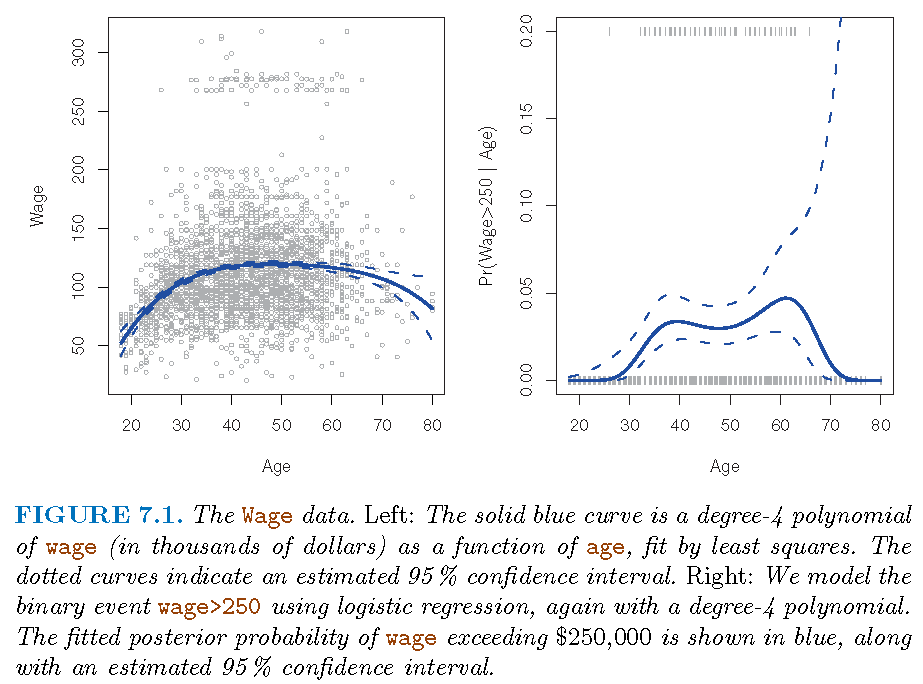
\includegraphics[width=0.85\linewidth]{fig7_1} \end{center}

\section{Regression splines}\label{regression-splines}

\subsection{Basis functions}\label{basis-functions}

\begin{itemize}
\item
  \(\left(d+1\right)\) monomials \(1,X,X^{2},...,X^{d}\) generate
  polynomials \(\mathcal{P}_d\) of degree \(d\) with elements: \[
  f_d(x)=\beta_{0}+\beta_{1}x+\beta_{2}x^{2}+\cdots+\beta_{d}x^{d}
  \]
\item
  \(d\) \textbf{functionally linearly independent} functions
  \(f_{1},...,f_{d}\) generate family \(\mathcal{F}\) with elements

  \begin{equation}
  \tilde{f}\left(  x\right)  =\beta_{0}+\beta_{1}f_{1}\left(  x\right)
  +\beta_{2}f_{2}\left(  x\right)  +\cdots+\beta_{d}f_{d}\left(  x\right)
  \end{equation}
\item
  \(\left\{ f_{i}\right\} _{i=1}^{d}\) are called
  \textquotedblleft basis functions\textquotedblright~for
  \(\mathcal{F}\)
\item
  Note: these are concepts in linear algebra
\end{itemize}

\subsection{Piecewise polynomials}\label{piecewise-polynomials}

\begin{itemize}
\item
  A \emph{global} polynomial regression model has intrinsic
  disadvantages
\item
  \textbf{Alternative strategy}: fit different polynomial regressions on
  different parts of data, by requiring these polynomials to be
  consistent in some sense, so that the \emph{resultant model displays
  some stability as it transits from one part of data to the other}
\item
  Consider the model \(M\): \[
  Y=\left\{
  \begin{array}
  [c]{cc}%
  \beta_{01}+\beta_{11}X+\beta_{21}X^{2}+\beta_{31}X^{3}, &  X<c\\
  \beta_{02}+\beta_{12}X+\beta_{22}X^{2}+\beta_{32}X^{3}, &  X\geq
  c
  \end{array}
  \right.
  \]
\end{itemize}

\subsection{Piecewise polynomials}\label{piecewise-polynomials-1}

\begin{itemize}
\item
  Data version \[
  y_{i}=\left\{
  \begin{array}
  [c]{cc}%
  \beta_{01}+\beta_{11}x_{i}+\beta_{21}x_{i}^{2}+\beta_{31}x_{i}^{3}, &  x_{i}<c\\
  \beta_{02}+\beta_{12}x_{i}+\beta_{22}x_{i}^{2}+\beta_{32}x_{i}^{3}, &  x_{i}\geq c
  \end{array}
  \right.
  \]
\item
  \(M\) has two sub-models, \(M_{1}\) and \(M_{2}\), on two distinct
  parts, \(D_{1}=\left\{ \left( X,Y\right) :X<c\right\}\) and
  \(D_{2}=\left\{ \left( X,Y\right) :X\geq c\right\}\), of data space
\item
  \(c\) for \(X\) is where \(M\) transits from \(M_{1}\) to \(M_{2}\)
  (or vice versa); \(c\) is called a ``knot''
\end{itemize}

\section{Splines: I}\label{splines-i}

\subsection{Splines}\label{splines}

\begin{itemize}
\tightlist
\item
  Splines are a type of regression polynomials:

  \begin{itemize}
  \tightlist
  \item
    They employ polynomials up to a fixed degree
  \item
    Where two polynomials meet, some constrains are satisfied
  \end{itemize}
\item
  \emph{Cubic splines} employ \(\deg(3)\) polynomials
\item
  \emph{Natural splines} also satisfy linear constraints at boundary
\item
  \textbf{Smoothing splines} directly satisfy smoothness constraints and
  need not to have polynomial components
\end{itemize}

\subsection{Cubic splines}\label{cubic-splines}

\begin{itemize}
\item
  Two cases of transition of \(M\) from \(M_{1}\) to \(M_{2}\):

  \begin{itemize}
  \tightlist
  \item
    Case 1: \(M_{1}\) does not match \(M_{2}\) at \(c\); e.g., \(M\)
    jumps from \(M_{1}\) to \(M_{2}\) at \(c\)
  \item
    Case 2: \(M_{1}\) matches \(M_{2}\) at \(c\) in some sense; e.g.,
    \(M_{1}\) matches \(M_{2}\) at \(c\), in value, (and/or) in speed of
    change, (and/or) in curvature
  \end{itemize}
\item
  For practical purposes it is often desirable to have Case 2, and the
  \(3\)-degree polynomials with matching values (i.e., \(M\) itself is
  continuous), speeds (i.e., first-order derivatives) and curvatures
  (i.e., second-order derivatives) at each knot are called \textbf{cubic
  splines}
\end{itemize}

\subsection{Illustration}\label{illustration}

\begin{center}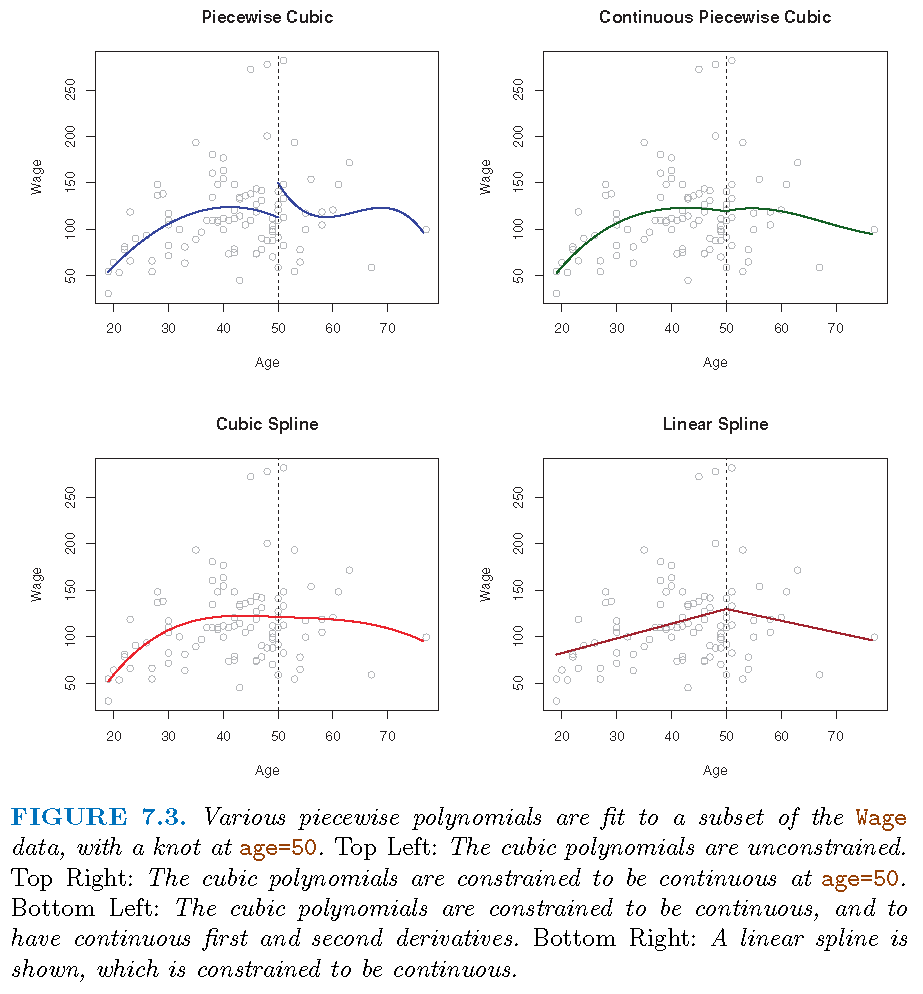
\includegraphics[width=0.8\linewidth]{fig7_3} \end{center}

\subsection{Smoothing splines}\label{smoothing-splines}

\begin{itemize}
\item
  Split the range of \(X\) into \(K+1\) parts and only employ
  polynomials of degree \(d\); so needing \(K\) knots and \(K+1\) such
  polynomials
\item
  Restrict these polynomials such that there are \(s\) constrains for
  each distinct pair of them at a knot, then we have \(p=T-C\)
  parameters to estimate
\item
  \(T = (K+1) \times (d+1)\); \((K+1)\) number of distinct regions of
  values of \(X\), and \(d+1\) number of parameters in each polynomial
\item
  \(C = K \times s\); \(K\) number of knots and \(s\) number of
  constraints at each knot
\end{itemize}

\subsection{Smoothing splines}\label{smoothing-splines-1}

In the above formula, \(s\), the number of constraints at each knot can
be understood as follows:

\begin{itemize}
\item
  If submodels \(M_{i}\) and \(M_{i+1},i=1,...,K\) match in their values
  and up to their \(\left( s-1\right)\)-th order derivatives at each
  knot \(Q_{i}\), then at knot \(Q_{i}\) there are \(s\) constraints on
  their associated polynomials
\item
  If we take \(0\)-th order derivative as performing no differentiation
  but keeping original function untouched, then \(M_{i}\) and
  \(M_{i+1},i=1,...,K\) matching up to their \(r\)-th order derivatives
  at each knot \(Q_{i}\) induces \(r+1\) constraints
\end{itemize}

\subsection{Smoothing splines:
representation}\label{smoothing-splines-representation}

\begin{itemize}
\item
  Consider \(d=3\). A cubic spline with \(K\) knots can be modelled as
  \[
  y_{i}=\beta_{0}+\beta_{1}b_{1}\left(  x_{i}\right)  +...+\beta_{K+3}b_{K+3}\left(  x_{i}\right)  +\varepsilon_{i}
  \] for an appropriate choice of basis functions
  \(b_{1},b_{2},...,b_{K+3}\)
\item
  One such basis is partially induced by the function \[
  h\left(  x,\xi\right)  =\left(  x-\xi\right)  _{+}^{3}=\left\{
  \begin{array}
  [c]{cc}%
  \left(  x-\xi\right)  ^{3}, & x>\xi\\
  0, & x\leq\xi
  \end{array}
  \right.
  \]
\end{itemize}

\subsection{Smoothing splines:
representation}\label{smoothing-splines-representation-1}

\begin{itemize}
\tightlist
\item
  In summary, to fit a cubic spline to a data set with \(K\) knots, we
  can equivalently fit the model \[
  Y=\beta_{0}+\beta_{1}X+\beta_{2}X^{2}+\beta_{3}X^{3}+\\
   \beta_{4}%
  \underbrace{h\left(  X,\xi_{1}\right)  }_{\text{the 4th predictor}}%
  +...+\beta_{K+3}h\left(  X,\xi_{K}\right)  +\varepsilon
  \] or its data version \[
  y_{i}=\beta_{0}+\beta_{1}x_{i}+\beta_{2}x_{i}^{2}+\beta_{3}x_{i}^{3}+\\
  \beta_{4}h\left(  x_{i},\xi_{1}\right)  +...+\beta_{K+3}h\left(  x_{i},\xi
  _{K}\right)  +\varepsilon_{i}
  \] where \(\xi_{1},...,\xi_{K}\) are the knots
\item
  Fitting this model uses \(K+4\) degrees of freedom. We can use the
  least squares method to fit the model
\end{itemize}

\subsection{Natural splines}\label{natural-splines}

\begin{itemize}
\item
  As for any regression that employs a polynomial, fitted model may be
  unstable near or at the boundary (induced by observed values of
  predictors)
\item
  A \textbf{natural spline} is a regression spline which is required to
  be \emph{linear at the boundary (in the region where \(X\) is smaller
  than the smallest knot, or larger than the largest knot)}
\end{itemize}

\subsection{Natural/Cubic spline}\label{naturalcubic-spline}

\begin{center}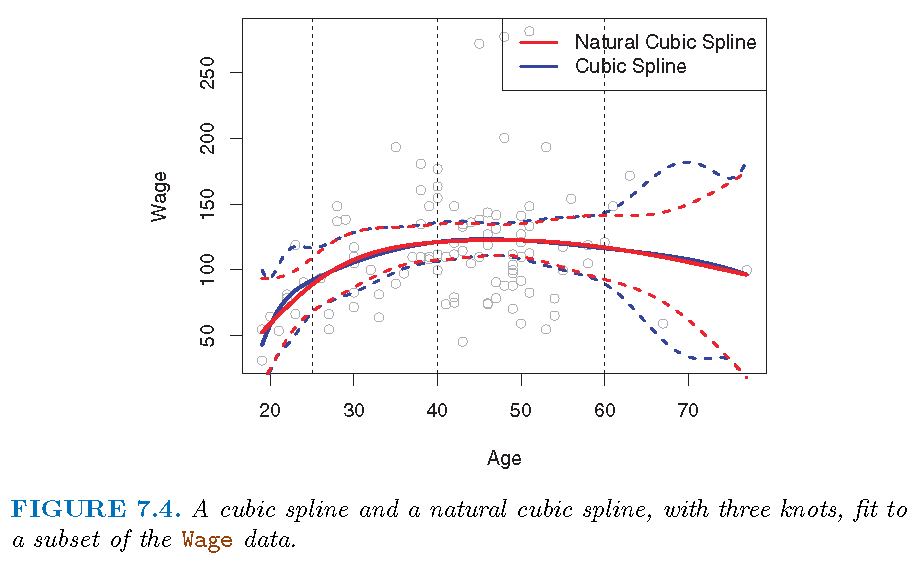
\includegraphics[width=0.85\linewidth]{fig7_4} \end{center}

\begin{itemize}
\tightlist
\item
  Each cubic spline has 3 knots
\end{itemize}

\section{Splines: II}\label{splines-ii}

\subsection{More knots?!}\label{more-knots}

\begin{itemize}
\item
  Regression spline is most flexible in regions that contain a lot of
  knots, because in those regions the polynomial coefficients can change
  rapidly. Hence, one option is to place more knots in places where we
  feel the function might vary most rapidly, and to place fewer knots
  where it seems more stable
\item
  While this option can work well, in practice it is common to place
  knots in a uniform fashion. One way to do this is to specify the
  desired degrees of freedom, and then have the software automatically
  place the corresponding number of knots at uniform quantiles of the
  data\textquotedblright, as done, e.g., by \emph{\(10\)-fold CV based
  on the residual sum of squares (RSS) values}
\end{itemize}

\subsection{Placing knots}\label{placing-knots}

\begin{center}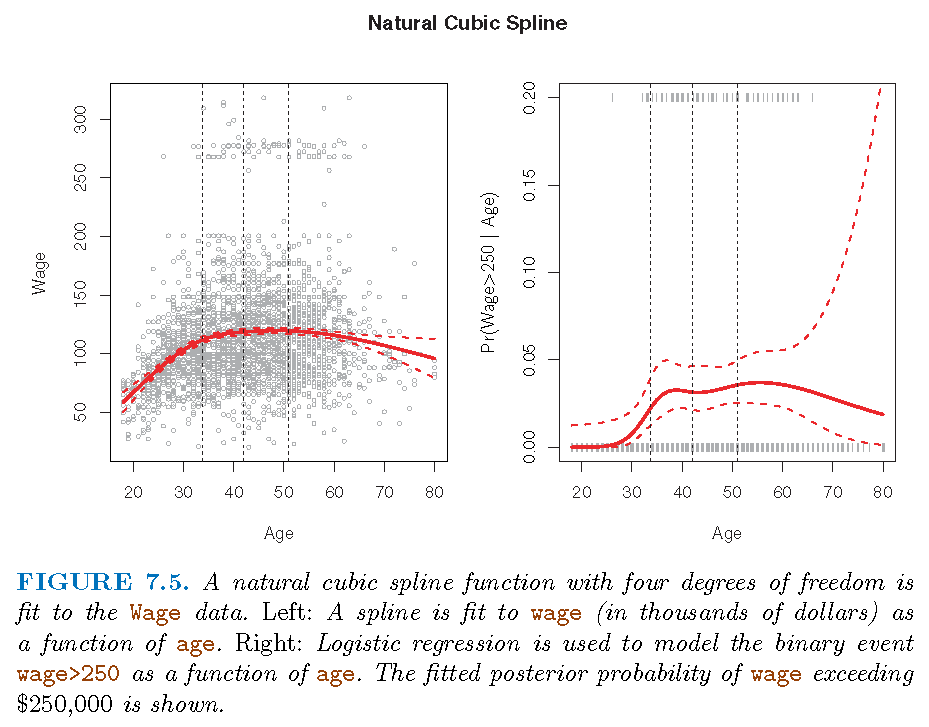
\includegraphics[width=0.85\linewidth]{fig7_5} \end{center}

\begin{itemize}
\tightlist
\item
  \(3\) knots, placed at 25th, 50th, 75th percentiles of \texttt{age}
\end{itemize}

\subsection{Choosing knots}\label{choosing-knots}

\begin{center}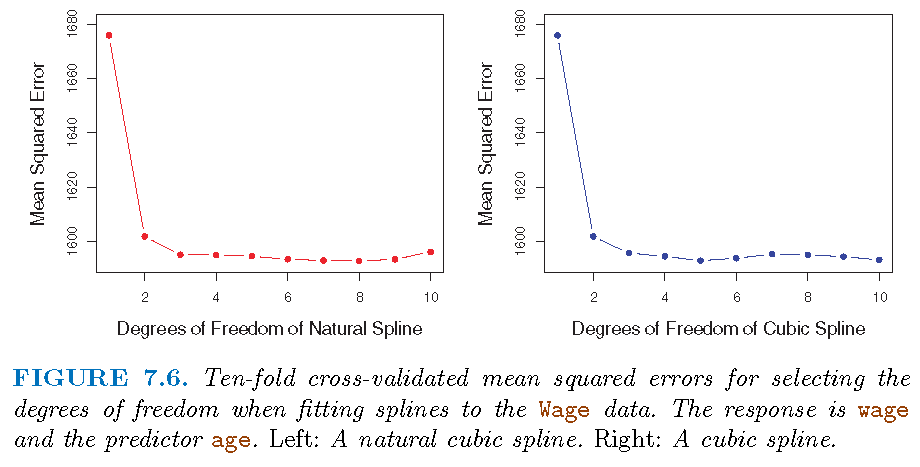
\includegraphics[width=0.85\linewidth]{fig7_6} \end{center}

\subsection{Comparison}\label{comparison}

``Regression splines often give superior results to polynomial
regression'':

\begin{itemize}
\item
  To be more flexible, polynomial regressions resort to higher degree
  polynomials which results in added instability at boundary (of
  observations for \(X\)).
\item
  Splines only need to plan for better knots in order to achieve
  flexibility, and natural splines alleviate instability at boundary
\item
  Spline captures much better (than polynomial regression) local
  behavior of \(f\) in true model \(E(Y|X)=f(X)\) where \(f\) changes
  rapidly.
\end{itemize}

\subsection{Illustration}\label{illustration-1}

\begin{center}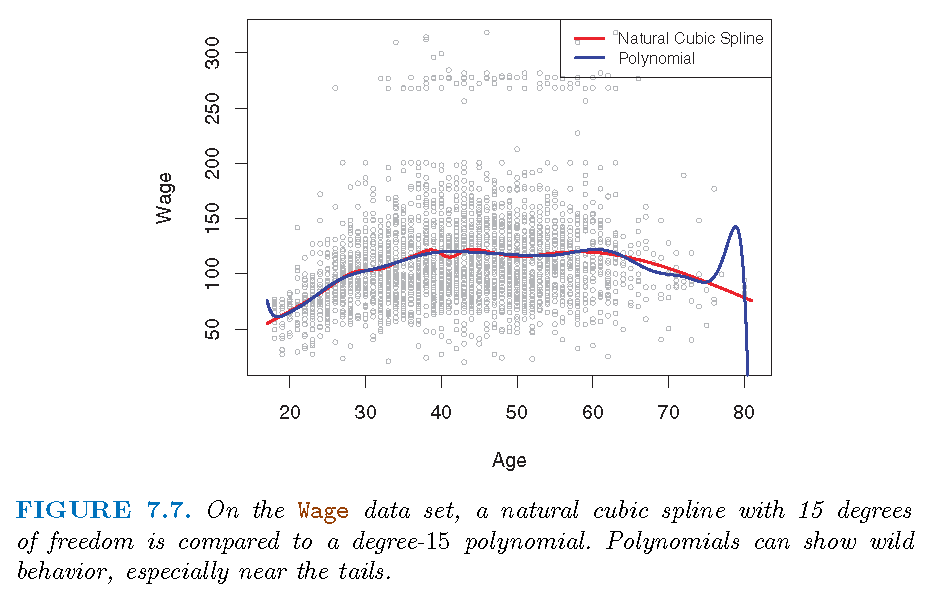
\includegraphics[width=0.85\linewidth]{fig7_7} \end{center}

\section{Smoothing splines}\label{smoothing-splines-2}

\subsection{Motivation}\label{motivation}

Smoothing splines are splines produced directly by restricting how
\textbf{smooth} a candidate function can be:

\begin{itemize}
\item
  Given the data
  \(\left\{ \left( x_{i},y_{i}\right) :i=1,...n\right\}\), there is a
  function \(g\) such that
  \(\sum_{i=1}^{n}\left( y_{i}-g\left( x_{i}\right) \right)^{2}=0\)
\item
  In terms of the local properties of \(g\) such as continuity and
  differentiability, we can restrict the \textquotedblleft integrated
  curvature of \(g\)\textquotedblright, which is
  \(\int\left[ g^{\prime\prime}\left( t\right) \right] ^{2}dt\). The
  integral essentially restricts how variable \(g^{\prime\prime}\) is
  (and hence approximately how variable the curvature of \(g\) is)
\end{itemize}

\subsection{Formulation}\label{formulation}

\begin{itemize}
\item
  A function \(g\) that minimizes

  \begin{equation}
  \underbrace{\sum_{i=1}^{n}\left(  y_{i}-g\left(  x_{i}\right)  \right)  ^{2}
  }_{\text{squared loss}}+\underbrace{\lambda\int\left[  g^{\prime\prime}\left(
  t\right)  \right]  ^{2}dt}_{\text{penalty on smoothness}} \label{eq76}%
  \end{equation}

  (for each fixed \(\lambda\geq0\)) is called a \emph{smoothing
  spline}\textquotedblright*
\item
  When is \(g^{\prime\prime}\left( t\right)\) a constant?
\item
  For practical usage, \(\deg\left( g\right) \ge 3\) if \(g\) is a
  polynomial
\item
  Penalty term referred to as \emph{roughness penalty}
\end{itemize}

\subsection{Key observations}\label{key-observations}

\begin{itemize}
\item
  When \(\lambda=0\), the penalty term has no effect and \(g\) can be
  discontinuous and will exactly interpolate the data
\item
  When \(\lambda\neq0\), \(g\) has to be twice differentiable in order
  to possess a second order derivative
\item
  When \(\lambda=\infty\), the minimizer \(\hat{g}\) must satisfy
  \(\hat{g}^{\prime\prime}\left( t\right) =0\). This means that
  \(\hat {g}\) has to be a linear function, i.e.,
  \(\hat{g}\left( x\right) =\beta _{0}+\beta_{0}x\), in which case we
  get linear regression
\end{itemize}

\subsection{Complexity and
performance}\label{complexity-and-performance}

The minimizer \(\hat{g}_{\lambda}\) for \(\lambda\in\left( 0,1\right)\),
being a shunken version of a natural cubic spline, has the following
properties:

\begin{itemize}
\item
  \(\hat{g}_{\lambda}\) is a piecewise cubic polynomial with knots at
  the unique values of \(x_{1},...,x_{n}\)
\item
  \(\hat{g}_{\lambda}\) has continuous first and second order
  derivatives at each knot
\item
  \(\hat{g}_{\lambda}\) is linear in the region outside of the extreme
  knots
\end{itemize}

\emph{Proof of the above is a bit complicated and uses machinery from
functional analysis and differential equations}

\subsection{Degrees of freedom}\label{degrees-of-freedom}

\begin{itemize}
\item
  Tuning parameter \(\lambda\) controls the \emph{effective degrees of
  freedom}, \(df_{\lambda}\), of \(\hat{g}\)
\item
  \(df_{\lambda}\) decreases from \(n\) to \(2\) as \(\lambda\)
  increases from \(0\) to \(\infty\)
\item
  \(df_{\lambda}\) measures flexibility of \(\hat {g}_{\lambda}\), in
  the sense that larger \(df_{\lambda}\) induces a more flexible
  \(\hat{g}_{\lambda}\)
\end{itemize}

\subsection{Degrees of freedom}\label{degrees-of-freedom-1}

\begin{itemize}
\item
  Let \(\mathbf{S}_{\lambda}\in\mathbb{R}^{n\times n}\) be formed by
  evaluating associated basis functions at the \(x_{i}\)'s. Then \[
  \mathbf{\hat{g}}_{\lambda}=\left(
  \begin{array}
  [c]{c}%
  \hat{g}_{\lambda}\left(  x_{1}\right)  \\
  \hat{g}_{\lambda}\left(  x_{2}\right)  \\
  \vdots\\
  \hat{g}_{\lambda}\left(  x_{n}\right)
  \end{array}
  \right)  =\mathbf{S}_{\lambda}\left(
  \begin{array}
  [c]{c}%
  y_{1}\\
  y_{2}\\
  \vdots\\
  y_{n}%
  \end{array}
  \right)
  \]
\item
  \textbf{Effective degrees of freedom} is defined as \[
  df_{\lambda}=\sum_{i=1}^{n}\mathbf{S}_{\lambda}\left(  i,i\right)  ,
  \] where \(\mathbf{S}_{\lambda}\left( i,j\right)\) is the
  \(\left( i,j\right)\) entry of \(\mathbf{S}_{\lambda}\)
\end{itemize}

\subsection{Choose tuning parameter}\label{choose-tuning-parameter}

\begin{itemize}
\item
  Best \(\lambda\) achieves the smallest cross-validation RSS among a
  grid values of \(\lambda\)
\item
  Quick computation via \emph{Leave-one-out-cross-validation (LOOCV)} in
  a single pass on the whole data: \[
  RSS_{cv}\left(  \lambda\right)  =\sum_{i=1}^{n}\left(  y_{i}-\hat{g}_{\lambda
  }^{\left(  -i\right)  }\left(  x_{i}\right)  \right)  ^{2}\\=\sum_{i=1}
  ^{n}\left[  \frac{y_{i}-\hat{g}_{\lambda}\left(  x_{i}\right)  }
  {1-\mathbf{S}_{\lambda}\left(  i,i\right)  }\right]  ^{2}
  \]

  \begin{itemize}
  \tightlist
  \item
    \(\hat{g}_{\lambda}^{\left( -i\right) }\): fitted on
    \(\left\{ \left( x_{j},y_{j}\right) :j\neq i\right\}\)
  \item
    \(\hat{g}_{\lambda}\): fitted on
    \(\left\{ \left( x_{i},y_{i}\right) :i=1,...,n\right\}\)
  \end{itemize}
\end{itemize}

\subsection{Illustration}\label{illustration-2}

\begin{center}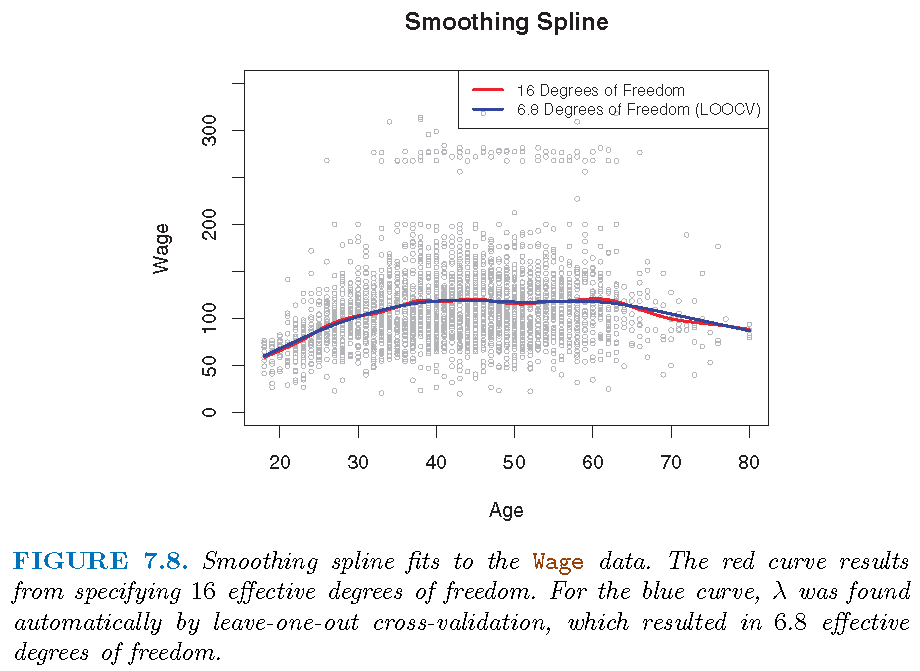
\includegraphics[width=0.85\linewidth]{fig7_8} \end{center}

\section{Generalized additive models}\label{generalized-additive-models}

\subsection{Overview}\label{overview-1}

\begin{itemize}
\item
  \emph{Generalized additive models (GAMs)} employs a non-linear
  function for each predictor while maintaining additivity of the
  transformed predictors
\item
  GAMs can be applied to both quantitative and qualitative responses
\item
  Consider \[
  y_{i}=\beta_{0}+\beta_{1}x_{i1}+\beta_{2}x_{i2}+\cdots+\beta_{p}%
  x_{ip}+\varepsilon_{i}
  \]
\item
  Replace \(\beta_{j}x_{ij}\) by \(f_{j}\left( x_{ij}\right)\) to get a
  GAM as \[
  y_{i}=\beta_{0}+f_{1}\left(  x_{i1}\right)  +f_{2}\left(  x_{i2}\right)
  +\cdots+f_{p}\left(  x_{ip}\right)  +\varepsilon_{i}
  \] for a set of known functions \(\left\{ f_{j}\right\} _{j=1}^{p}\)
\end{itemize}

\subsection{Illustration: I}\label{illustration-i}

\begin{itemize}
\tightlist
\item
  \(f_{1}\) and \(f_{2}\) natural splines; \(f_{3}\) piecewise constant:
  \[
  \text{wage }=\text{ }\beta_{0}+f_{1}\left(  \text{year}\right)  +f_{2}\left(
  \text{age}\right)  +f_{3}\left(  \text{education}\right)  +\varepsilon
  \]
\end{itemize}

\begin{center}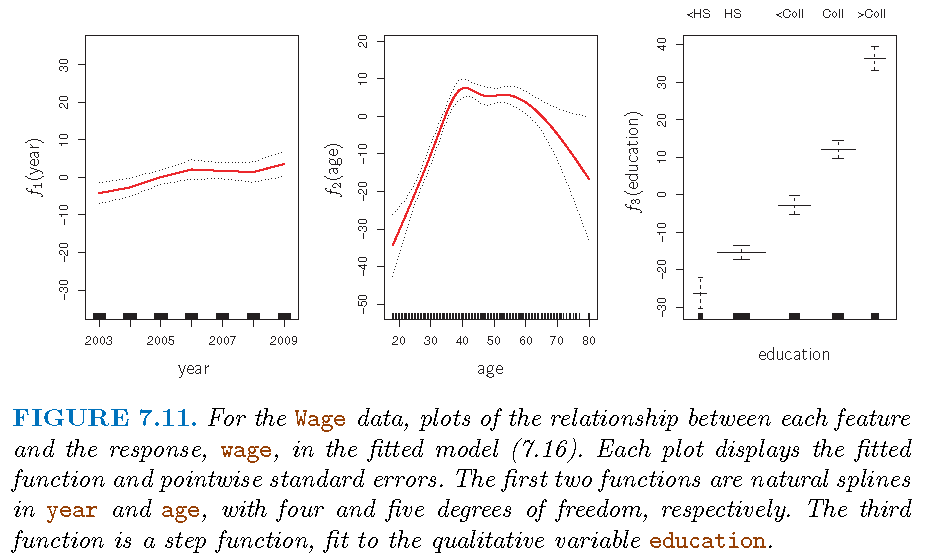
\includegraphics[width=0.85\linewidth]{fig7_11} \end{center}

\subsection{Illustration: II}\label{illustration-ii}

\begin{center}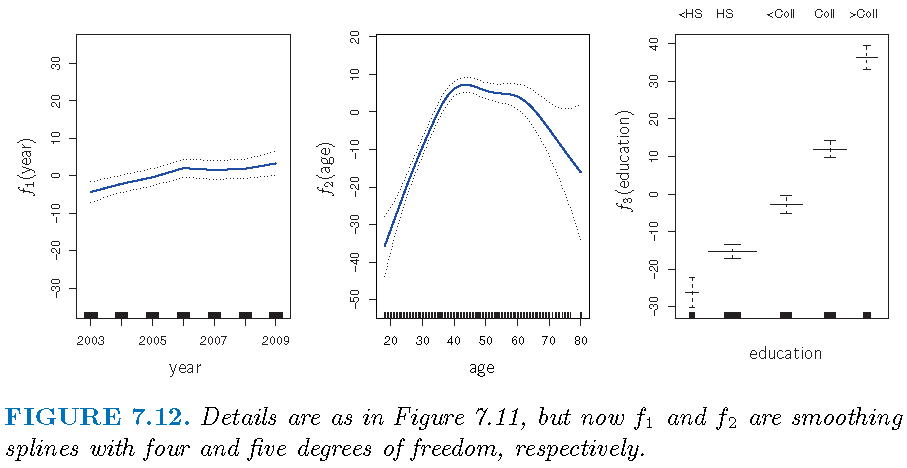
\includegraphics[width=0.85\linewidth]{fig7_12} \end{center}

\subsection{GAM logistic Reg}\label{gam-logistic-reg}

\begin{itemize}
\item
  A binary response, linear version: \[
  \log\left(  \frac{\Pr\left(  Y=1|X\right)  }{1-\Pr\left(  Y=1|X\right)
  }\right) \\ =\beta_{0}+\beta_{1}x_{i1}+\beta_{2}x_{i2}+\cdots+\beta_{p}%
  x_{ip}+\varepsilon_{i}%
  \]
\item
  GAM version: \[
  \log\left(  \frac{\Pr\left(  Y=1|X\right)  }{1-\Pr\left(  Y=1|X\right)
  }\right)  \\=\beta_{0}+f_{1}\left(  x_{i1}\right)  +f_{2}\left(  x_{i2}\right)
  +\cdots+f_{p}\left(  x_{ip}\right)  +\varepsilon_{i}%
  \]
\end{itemize}

\subsection{Illustration: III}\label{illustration-iii}

\begin{itemize}
\item
  Predict \[p\left(  X\right)  =\Pr\left(  \text{wage}
  >250|\text{year,age,education}\right)\]
\item
  Model: \[
  \log\left(  \frac{p\left(  X\right)  }{1-p\left(  X\right)  }\right)
  \\ =\beta_{0}+\beta_{1}\times\text{year}+f_{2}\left(  \text{age}\right)
  +f_{3}\left(  \text{education}\right)
  \]
\item
  Note: there are no individuals with less than a high school education
  who earn over \$250,000 per year
\end{itemize}

\subsection{Illustration: III}\label{illustration-iii-1}

\begin{center}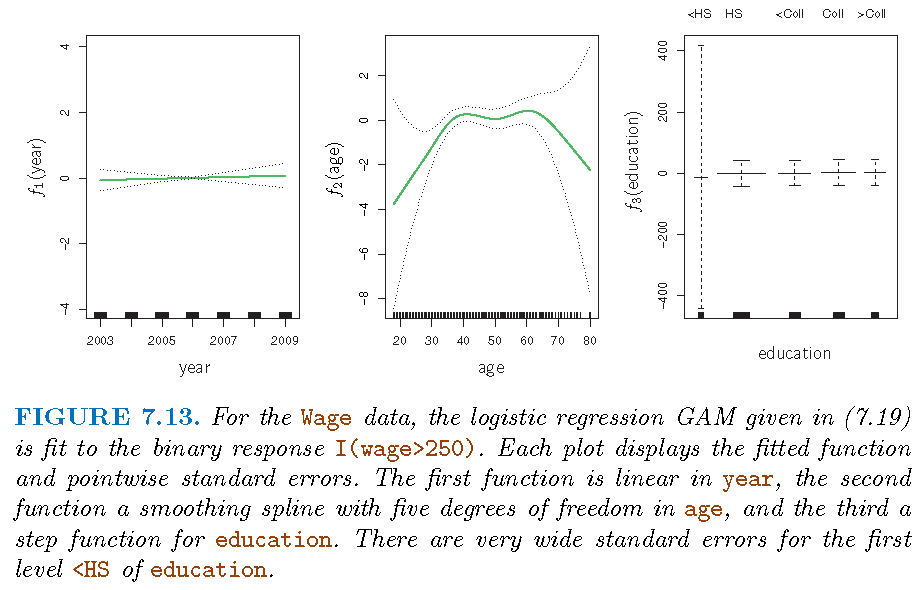
\includegraphics[width=0.85\linewidth]{fig7_13} \end{center}

\begin{itemize}
\tightlist
\item
  GAMs are implemented by R library \texttt{gam}
\end{itemize}

\subsection{License and session
Information}\label{license-and-session-information}

\href{http://math.wsu.edu/faculty/xchen/stat412/LICENSE.html}{License}

\begin{Shaded}
\begin{Highlighting}[]
\NormalTok{>}\StringTok{ }\KeywordTok{sessionInfo}\NormalTok{()}
\NormalTok{R version }\FloatTok{3.5.0} \NormalTok{(}\DecValTok{2018-04-23}\NormalTok{)}
\NormalTok{Platform:}\StringTok{ }\NormalTok{x86_64-w64-mingw32/}\KeywordTok{x64} \NormalTok{(}\DecValTok{64}\NormalTok{-bit)}
\NormalTok{Running under:}\StringTok{ }\NormalTok{Windows }\DecValTok{10} \KeywordTok{x64} \NormalTok{(build }\DecValTok{19044}\NormalTok{)}

\NormalTok{Matrix products:}\StringTok{ }\NormalTok{default}

\NormalTok{locale:}
\NormalTok{[}\DecValTok{1}\NormalTok{] LC_COLLATE=English_United States}\FloatTok{.1252} 
\NormalTok{[}\DecValTok{2}\NormalTok{] LC_CTYPE=English_United States}\FloatTok{.1252}   
\NormalTok{[}\DecValTok{3}\NormalTok{] LC_MONETARY=English_United States}\FloatTok{.1252}
\NormalTok{[}\DecValTok{4}\NormalTok{] LC_NUMERIC=C                          }
\NormalTok{[}\DecValTok{5}\NormalTok{] LC_TIME=English_United States}\FloatTok{.1252}    

\NormalTok{attached base packages:}
\NormalTok{[}\DecValTok{1}\NormalTok{] stats     graphics  grDevices utils     datasets  methods  }
\NormalTok{[}\DecValTok{7}\NormalTok{] base     }

\NormalTok{other attached packages:}
\NormalTok{[}\DecValTok{1}\NormalTok{] knitr_1}\FloatTok{.21}

\NormalTok{loaded via a }\KeywordTok{namespace} \NormalTok{(and not attached):}
\StringTok{ }\NormalTok{[}\DecValTok{1}\NormalTok{] compiler_3}\FloatTok{.5.0}  \NormalTok{magrittr_1}\FloatTok{.5}    \NormalTok{tools_3}\FloatTok{.5.0}    
 \NormalTok{[}\DecValTok{4}\NormalTok{] htmltools_0}\FloatTok{.3.6} \NormalTok{yaml_2}\FloatTok{.2.0}      \NormalTok{Rcpp_1}\FloatTok{.0.12}    
 \NormalTok{[}\DecValTok{7}\NormalTok{] stringi_1}\FloatTok{.2.4}   \NormalTok{rmarkdown_1}\FloatTok{.11}  \NormalTok{stringr_1}\FloatTok{.3.1}  
\NormalTok{[}\DecValTok{10}\NormalTok{] xfun_0}\FloatTok{.4}        \NormalTok{digest_0}\FloatTok{.6.18}   \NormalTok{evaluate_0}\FloatTok{.13}  
\end{Highlighting}
\end{Shaded}


\end{document}
